\documentclass{ctexart}

\usepackage{amsmath}
\usepackage{graphicx}
\usepackage{float}
\usepackage{listings}
\usepackage{xcolor}

\lstset{
    basicstyle=\ttfamily\small,
    keywordstyle=\color{blue},
    commentstyle=\color{gray},
    stringstyle=\color{red},
    showstringspaces=false,
    frame=single,      % 单线边框
    numbers=left,      % 行号在左侧
    numberstyle=\tiny\color{gray}
}

\title{ailab}
\author{ }
\date{\today}

\begin{document}
\maketitle
\tableofcontents
\newpage

\section{环境准备(WSL 下)}
\subsection{基础python环境}
\textbf{安装curl}\\
\verb|sudo apt install -y curl|\\

\textbf{安装uv}\\
\verb!curl -LsSf https://astral.sh/uv/install.sh | sh!\\

\textbf{更新python}\\
\verb|uv python install 3.12|\\

\subsection{训练工具}
\textbf{激活虚拟环境}\\
\verb|source .venv/bin/activate|, 终端出现\verb|(.venv)|前缀\\

\textbf{安装pytorch}\\
\verb|uv pip install torch torchvision torchaudio|\\
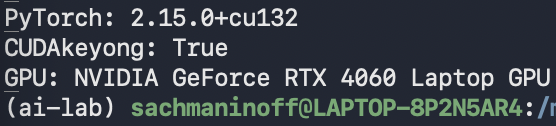
\includegraphics[width = 0.5\textwidth]{torch.png}\\

\textbf{安装trl}\\
\verb|python -m ensurepip --upgrade|\\
\verb|python -m pip trl|\\

\subsection{网络环境}

\textbf{pip换源}\\
\verb|pip config|位于:\verb|~/.config/pip/pip.conf|, 添加:\\
\begin{verbatim}
[global]
index-url = https://pypi.tuna.tsinghua.edu.cn/simple
trusted-host = pypi.tuna.tsinghua.edu.cn
\end{verbatim}

\textbf{wsl代理}\\
本机已经使用socks5代理, 监听端口8888, 只需要设置bash代理端口, 在~/.bashrc中添加:
\begin{verbatim}
export ALL_PROXY="socks5h://127.0.0.1:8888"
export all_proxy="$ALL_PROXY"
\end{verbatim}

\textbf{python socks代理支持}\\
注意此时的pip还不能使用代理, 所以加上env -u暂时禁用代理\\
\verb|env -u ALL_PROXY -u all_proxy python -m pip install socksio|

\subsection{尝试运行第一个程序}




\section{实验一}
a

\end{document}